\documentclass[a4paper]{report}

\usepackage{fontspec}				% utf-8 support
\usepackage{graphicx}				% To include images
\usepackage[margin=2.5cm]{geometry}	% Better margins
\usepackage[catalan]{babel}			% Catalan sections support
\usepackage[hidelinks]{hyperref}	% Autoref support
\usepackage{setspace}				% Allows to set a specific stretch

\addto\captionscatalan{\renewcommand{\chaptername}{Pràctica}}

\setlength{\parindent}{0pt}
\setlength{\parskip}{0.2cm}

\title{\textsc{\huge Tecnologia de Selecció de Materials} \\
        Informe pràctiques}
\author{Marta Gomis Domènech \and 
    Joan Marcè Igual \and 
    Èlia Mateu Barriendos \and 
    Esteve Tarragó Sanchís \and 
    Néstor Tuneu Arroyo}

\begin{document}

\begin{titlepage}
    \centering
    \vspace{1cm}
    
\includegraphics[width=0.25\textwidth]{images/etseib}
    \par\vspace{1cm}
    \textsc{ \LARGE Escola Tècnica Superior d'Enginyeria \\[1em] 
        Industrial de Barcelona}
    \par\vspace{2cm}
    \textbf{\Huge Tecnologia i Selecció de Materials}
    \par\vspace{2cm}
    {\LARGE Informe pràctiques}
    \vfill
    \begin{flushright}
        \large
        Marta Gomis Domènech \par
        Joan Marcè Igual \par
        Èlia Mateu Barriendos \par
        Esteve Tarragó Sanchís \par
        Néstor Tuneu Arroyo
    \end{flushright}
\end{titlepage}

\tableofcontents

\chapter{Assaig a tracció}

\section{Proveta metà\l. lica }

La \autoref{fig:traccio-metalica-grafic-proveta} correspon al resultat de l’assaig a tracció de la proveta metà\l.lica de 6 mm de diàmetre inicial, marcada amb separacions de 10 mm per estimar posteriorment paràmetres de ruptura. 

\begin{figure}[hb]
    \centering
    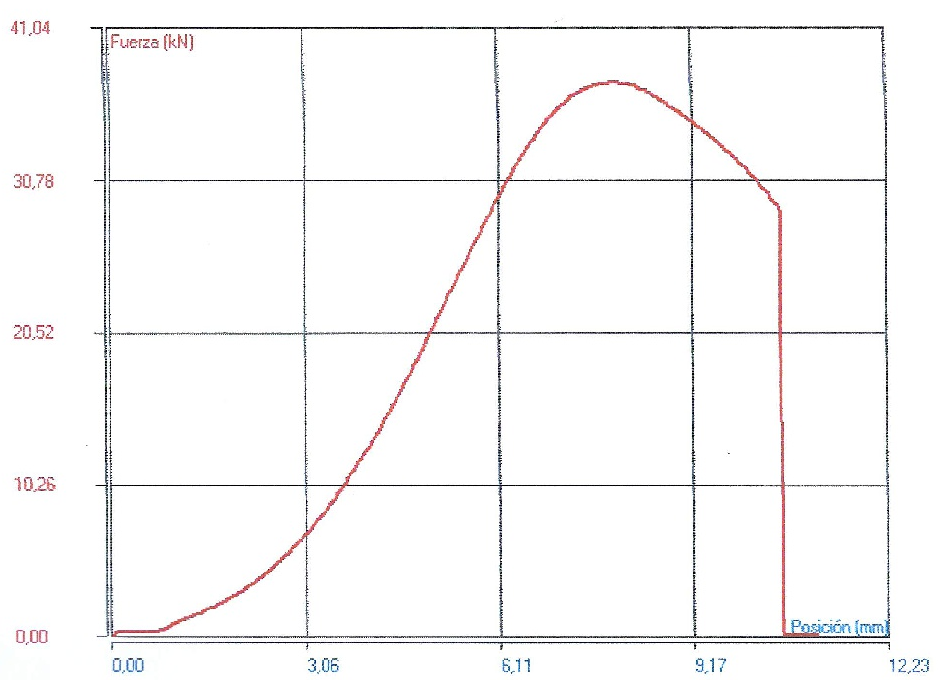
\includegraphics[width=0.9\textwidth]{images/traccio/metalica-grafic-proveta}
    \caption{Gràfic F-d de la proveta metà\l.lica}
    \label{fig:traccio-metalica-grafic-proveta}
\end{figure}

Abans de concretar algunes qüestions sobre l’assaig, a priori ja es poden extreure algunes conclusions del únicament utilitzant el gràfic:
\begin{itemize}
    \item  S’ha produït la ruptura del material. Això ho poden notar amb la línia vertical final en el gràfic.
    \item  La peça ha relliscat al principi, com queda indicat a la línia horitzontal inicial del gràfic. Aquest fenomen retarda l’aparició de la zona elàstica del material, caracteritzada per una zona de pendent constant, que es troba aproximadament entre els 4 mm i els 6,11 mm de desplaçament dels capçals de la màquina.
    \item  El material ha patit estricció. La zona de pendent negatiu indica que la secció del material està disminuint, doncs es necessita menys força per continuar deformant.
    \item  La ruptura és dúctil. Es pot corroborar analitzant la superfície de ruptura.
\end{itemize}

\subsection{El fenomen de l'estricció}

Durant l’assaig a tracció, en superar el valor màxim de força, el material plastifica i comença a deformar apareixent un coll. Aquesta deformació axial genera una contracció radial que redueix la secció de la proveta. La màquina d’assaigs a tracció, aplica força per moure’s a velocitat constant, per tant, com la secció disminueix aplica menys força per continuar deformant a la mateixa velocitat, fins arribar a la fallida per ruptura de la peça.

A la \autoref{fig:traccio-metalica-grafic-proveta} això es tradueix en una regió de pendent negativa entre el valor màxim de força i el moment de la fallida, tal com s’ha comentat al principi.

Com el material és crista\l.lí, el material no deforma gaire abans de trencar.

\subsection{Morfologia de la fractura}
Per estudiar la morfologia de la ruptura és essencial la fixar-se en la superfície de fractura. El primer que s’observa en una de les parts és un contorn ondulat que indica que el material ha deformat abans de trencar i per tant la ruptura és dúctil. Aquest contorn ondulat té major diàmetre que el diàmetre d’estricció màxima, per tant, es pot concloure que aquest fragment ha fallat per forces tangencials, abans de trencar definitivament.

Un altre indicador de ruptura dúctil és la rugositat de les superfícies, que s’observa a ull nu malgrat la contaminació d’aquestes. De tota manera, les peces encaixen amb relativa facilitat, per tant el material no deforma de manera considerable com els polímers, dels quals es parlarà més endavant.

Aquestes consideracions es veuen i\l.lustrades a la \autoref{fig:traccio-metalica-superficie-ruptura}, que és una fotografia de les dues superfícies de ruptura. 

\begin{figure}[ht]
    \centering
    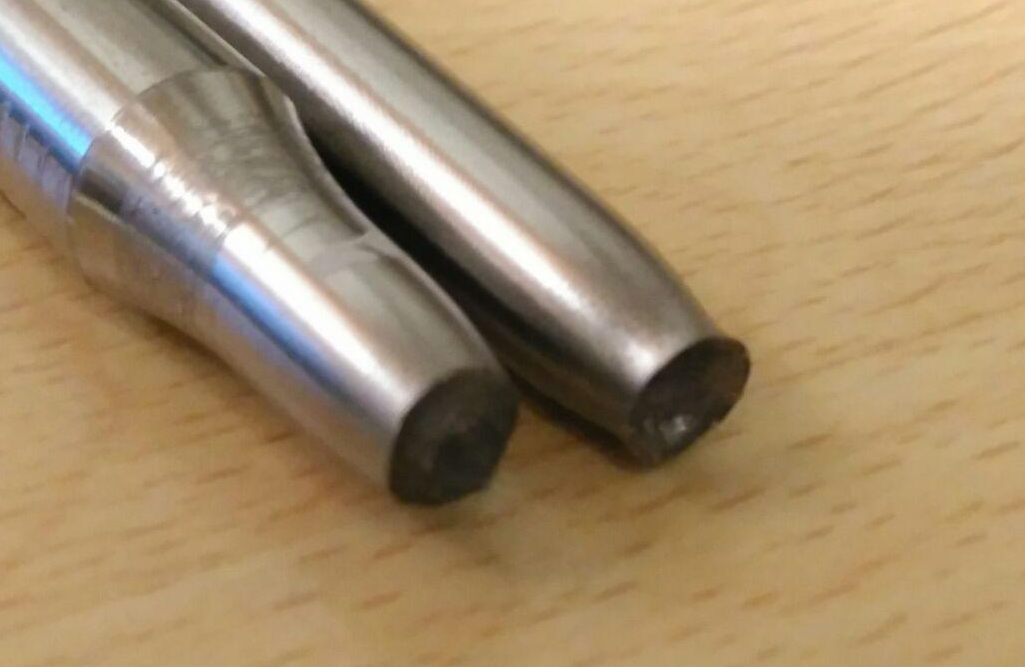
\includegraphics[width=0.5\textwidth]{images/traccio/metalica-superficie-ruptura}
    \caption{Superfícies de ruptura de la proveta metà\l.lica}
    \label{fig:traccio-metalica-superficie-ruptura}
\end{figure}

\subsection{Paràmetres de ruptura}

Utilitzant les marques inicials de la proveta, les dimensions finals i el gràfic F-d, es poden obtenir els següents paràmetres: límit elàstic, càrrega màxima, allargament a la ruptura (\%) i estricció (\%).

La càrrega màxima és una mesura directa del gràfic, sent el màxim valor d’aquesta. Mitjançant mètodes d’aproximació gràfica, s’ha estimat que aquest valor és $38,43 \ kN$.

El límit elàstic real es defineix com el punt on el material comença a plastificar. El límit elàstic convencional tolera un $0,2\%$ de deformació. Aquests dos valors són representatius del valor del límit elàstic i es poden estimar sempre que es puguin mesurar les deformacions. 

Donat que no es disposava d’extensòmetre es farà l’aproximació del valor del límit elàstic com el quocient entre el valor de força abans d’abandonar el règim elàstic entre l’àrea inicial. Aprofitant que les deformacions en la proveta metà\l.lica són reduïdes, s’ha considerat que és una estimació suficientment correcte.

S’ha pres el valor de força (estimat també gràficament) de $28,50 \ kN$, el que suposa una tensió de límit elàstic de $1007,98 \ N/mm^2$. S’ha suposat que la secció de la proveta és perfectament circular.

Quant a l’allargament a la ruptura, la distància entre les marques entre les quals s’ha produït la ruptura ha passat de $10 \ mm$ a $13,6 \ mm$, per tant, l’allargament és d’un $36\%$.

Per últim, el diàmetre final de la proveta, mesurada amb una precisió de $0,1 \ mm$ és de $5 \ mm$, per tant, l’estricció és d’un $30,56\%$.



\end{document}